\documentclass[conference]{IEEEtran}
\usepackage[utf8]{inputenc}
\usepackage[T1]{fontenc}
\usepackage{amsmath,amssymb}
\usepackage{booktabs}
\usepackage{graphicx}
\usepackage{multirow}
\usepackage{xcolor}
\usepackage{algorithm}
\usepackage{algpseudocode}
\usepackage[hidelinks]{hyperref}
\usepackage{cite}

% Tables and figures are generated by the evaluation scripts into ../results; until a file
% exists a placeholder box is shown, so the report always compiles.
\newcommand{\resultstable}[1]{\IfFileExists{../results/tables/#1.tex}{\input{../results/tables/#1.tex}}%
  {\fbox{\parbox{0.92\columnwidth}{\centering\small\itshape Generated table \texttt{\detokenize{#1}} not available yet.}}}}
\newcommand{\resultsfigure}[2][\columnwidth]{\IfFileExists{../results/figures/#2.png}%
  {\includegraphics[width=#1]{../results/figures/#2.png}}%
  {\fbox{\parbox{0.92\columnwidth}{\centering\small\itshape Generated figure \texttt{\detokenize{#2}} not available yet.}}}}
\newcommand{\pending}[1]{\textcolor{gray}{[\emph{#1}]}}
\newcommand{\cmi}{\mathrm{CMI}}

\begin{document}

\title{Enhancing Multi-Agent Emotional Support Conversations for Code-Mixed Hinglish Help-Seekers with Cross-Lingual Experience Retrieval and Register-Aware Response Selection}

\author{\IEEEauthorblockN{Roshan Raj (12341830)}
\IEEEauthorblockA{Indian Institute of Technology Bhilai\\
roshanr@iitbhilai.ac.in}}

\maketitle

\begin{abstract}
MultiAgentESC is a recent multi-agent framework for emotional support conversation (ESC) in which
LLM agents analyse the help-seeker's state, deliberate on support strategies with retrieved
similar cases, and debate to select a response. It is designed, prompted and evaluated for
English only, while many help-seekers in India express distress in code-mixed Hindi--English
(Hinglish). We present CodeMixESC, which keeps the three-stage pipeline and adds four components
without fine-tuning the LLM agents: a Code-Mix Profiler that measures the seeker's register with
word-level language identification and the Code-Mixing Index (CMI); a cross-lingual experience
retriever, a multilingual sentence encoder fine-tuned contrastively on Hinglish--English pairs so
that Hinglish queries retrieve the English case bank without translating it; register-aware
generation and selection, which adds a language and cultural fit criterion to debate, voting and
refinement; and a Register Gate that re-refines a response whose CMI departs from the seeker's by
more than a tuned threshold, adding at most one LLM call per turn. We also build ESConv-HiEn, a
parallel Roman-script Hinglish version of the ESConv test set at two mixing levels that keeps the
strategy labels, enabling a controlled robustness study. \pending{One or two sentences with the
main results are added once the experiments in Section~\ref{sec:results} are complete.}
\end{abstract}

\section{Introduction}
Mental health care in India faces a severe shortage of professionals; the National Mental Health
Survey 2015--16 reported a treatment gap of more than 60\% for almost every mental disorder
\cite{gururaj2016nmhs}. Emotional Support Conversation (ESC) systems \cite{liu2021towards} aim to
reduce this gap with dialogue agents that comfort people using professional support strategies
such as \emph{Question}, \emph{Reflection of feelings} and \emph{Providing Suggestions}.
MultiAgentESC \cite{xu2025multiagentesc} is a strong recent system in this line: specialised LLM
agents analyse the user's psychological state, deliberate on strategies using retrieved similar
cases, and debate to select the best response.

People express emotions most authentically in their preferred language \cite{srivastava2026knowledge},
and for many Indian users this is Hinglish typed in Roman script, e.g.\ \emph{``yaar result aaya,
bahut tension ho rahi hai, ghar pe kaise bataun''}. Recent benchmarks show that LLMs still
struggle to reason about and generate code-switched text \cite{winata2026codeswitch}. For such
users MultiAgentESC retrieves its experience with an English-only encoder, selects and refines
responses without considering the user's register, and has never been evaluated on code-mixed
input. Code-mixing is a realistic distribution shift: handling it requires cross-lingual
representation learning, robustness evaluation under a controlled shift, and generation towards a
measurable target, the language mix.

\noindent\textbf{Contributions.} (i) CodeMixESC, which extends MultiAgentESC with a Code-Mix
Profiler, a contrastively fine-tuned cross-lingual retriever, register-aware generation and
selection, and a Register Gate (Section~\ref{sec:method}); (ii) ESConv-HiEn, a parallel Hinglish
version of the ESConv test set at two mixing levels with strategy labels
(Section~\ref{sec:data}); (iii) a controlled evaluation of retrieval robustness, response quality,
register match, strategy stability and efficiency against prompting baselines, MultiAgentESC and a
translate-pivot pipeline, with ablations (Sections~\ref{sec:setup}--\ref{sec:results}).

\section{Related Work}
\textbf{Emotional support conversation.} ESConv \cite{liu2021towards} defines eight support
strategies and provides strategy-annotated conversations. MultiAgentESC
\cite{xu2025multiagentesc} organises LLM agents with AutoGen \cite{wu2024autogen} into dialogue
analysis, strategy deliberation with retrieved cases (Sentence-BERT \cite{reimers2019sbert}), and
response generation with debate, reflection and voting.
\textbf{Code-mixed NLP and mental health.} HingBERT \cite{nayak2022hingbert} provides Hinglish
language models and a word-level language identifier; PHINC \cite{srivastava2020phinc} is a
parallel Hinglish--English corpus. Srivastava et al.\ \cite{srivastava2026knowledge} introduce a
Hinglish counselling dataset but only perform emotion recognition; Kumar and Chakraborty
\cite{kumar2024harmonizing} generate code-mixed responses in general conversations without
support strategies. To the best of our knowledge no prior work studies strategy-based emotional
support generation for code-mixed help-seekers.
\textbf{Cross-lingual sentence embeddings.} Multilingual Sentence-BERT models are obtained by
knowledge distillation \cite{reimers2020multilingual}; LaBSE \cite{feng2022labse} is trained on
translation pairs. Contrastive training with in-batch negatives \cite{henderson2017smartreply} is
the standard way to adapt such encoders to a new pair of domains.
\textbf{Register accommodation.} Communication Accommodation Theory \cite{giles1991accommodation}
holds that converging towards a partner's speech style builds rapport, while diverging creates
social distance, which motivates matching the seeker's language mix.

\section{Method}\label{sec:method}
CodeMixESC keeps the three stages of MultiAgentESC (Fig.~\ref{fig:pipeline}): (i) dialogue
analysis, where a decision maker judges whether the dialogue reflects the user's emotion, its
cause and the user's coping intention, and if so emotion, cause and intention agents analyse it;
(ii) strategy deliberation, where three agents choose strategies in a round-robin group chat over
the ten most similar ESConv cases; (iii) response generation, where one response per strategy is
debated, reflected on and voted for, a judge breaks ties, and a refiner polishes the winner.
Early turns and non-complex dialogues are answered by a single zero-shot agent. The decision
maker, the deliberation prompt and the judge are unchanged.

\begin{figure}[t]
\centering
\IfFileExists{figures/pipeline.pdf}{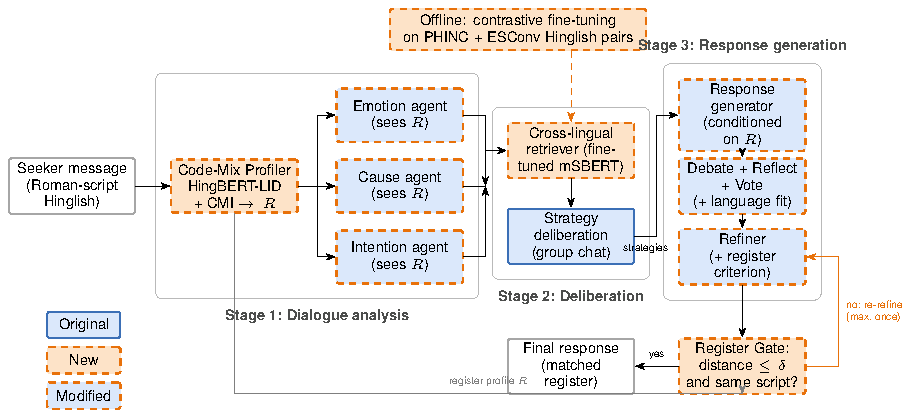
\includegraphics[width=\columnwidth]{figures/pipeline.pdf}}{%
\fbox{\parbox{0.92\columnwidth}{\small Seeker message $\rightarrow$ \textbf{Code-Mix Profiler} (R)
$\rightarrow$ decision maker $\rightarrow$ emotion/cause/intention agents (+R) $\rightarrow$
\textbf{cross-lingual retriever} $\rightarrow$ strategy deliberation $\rightarrow$ response per
strategy (+R) $\rightarrow$ debate, reflection, vote (+language fit) $\rightarrow$ judge
$\rightarrow$ refiner (+register) $\rightarrow$ \textbf{Register Gate} $\rightarrow$ response.}}}
\caption{CodeMixESC. Components in bold are new; components marked +R are modified to receive
the seeker's register profile R.}
\label{fig:pipeline}
\end{figure}

\subsection{Code-Mix Profiler}
Every seeker utterance is tagged word by word with HingBERT-LID \cite{nayak2022hingbert}; numbers,
punctuation, emojis, URLs, mentions and hashtags are language independent, and Devanagari words
are Hindi by script. The Code-Mixing Index \cite{gamback2016cmi} is
\begin{equation}
\cmi = \begin{cases} 1 - \dfrac{\max_i w_i}{n-u}, & n > u\\[4pt] 0, & n = u\end{cases}
\end{equation}
where $w_i$ is the number of words of language $i$, $n$ the number of tokens and $u$ the number of
language-independent tokens. Because a single short reply (``yes'') gives an unstable CMI, the
profile is pooled over all seeker utterances so far (each utterance is tagged separately, and long
texts are processed in chunks so that no word is truncated). The profiler outputs the register
profile $R = (\cmi_s, \text{dominant language}, \text{script})$, which every later agent receives
together with an instruction to interpret common Hinglish distress expressions (\emph{tension},
\emph{ghabrahat}, \emph{log kya kahenge}) in context rather than literally.

\subsection{Cross-lingual experience retrieval}
The base system encodes the seeker's last message with the English encoder all-roberta-large-v1
and retrieves the ten most similar seeker posts of the English case bank (13,484 post--response
pairs of the ESConv training conversations). We replace it with
paraphrase-multilingual-mpnet-base-v2 \cite{reimers2020multilingual}, fine-tuned on
Hinglish--English pairs $(h_i, e_i)$ with the Multiple Negatives Ranking loss
\cite{henderson2017smartreply}
\begin{equation}
\mathcal{L} = -\frac{1}{B}\sum_{i=1}^{B}\log\frac{\exp(\cos(h_i,e_i)/\tau)}{\sum_{j=1}^{B}\exp(\cos(h_i,e_j)/\tau)},
\end{equation}
where $B$ is the batch size and $\tau$ a temperature. Training pairs come from PHINC
\cite{srivastava2020phinc} and from ESConv training utterances rewritten into Hinglish by an LLM
(Section~\ref{sec:data}). The English case bank is encoded once with the new model, so English
experience is reused for Hinglish queries without translating the case bank.

\subsection{Register-aware generation and selection}
The response generator receives $R$ and the instruction to reply ``in the same script with a
similar Hindi--English mix'' while keeping the assigned strategy and the 30-word limit; the
retrieved English examples are marked as illustrations of the strategy only. Debate, reflection
(the voting round) and the refiner add a fourth criterion, \emph{language and cultural fit}:
``Does the response match the seeker's language, script and level of Hindi--English mixing, and
does it sound natural?'', so that a well-written but register-mismatched candidate can lose the
vote. The single-agent path receives the same register instruction.

\subsection{Register Gate}
After refinement the gate measures the response's $\cmi_r$ and script
(Algorithm~\ref{alg:gate}). If $|\cmi_r-\cmi_s|>\delta$ or the script differs, the response is
rewritten once with an explicit register instruction that states the measured mismatch. The
rewrite is kept only if its register is closer to the seeker's, so the gate can never worsen the
match, and it adds at most one LLM call per turn. $\delta$ is tuned on a development set.

\begin{algorithm}[t]
\caption{Register Gate}\label{alg:gate}
\begin{algorithmic}[1]
\Require response $y$, strategy $s$, seeker profile $R$, threshold $\delta$
\State $r \gets \textsc{Profile}(y)$
\If{$|\cmi_r - \cmi_s| \le \delta$ \textbf{and} $\text{script}_r = \text{script}_s$} \Return $y$ \EndIf
\State $y' \gets \textsc{LLM}(\text{rewrite } y \text{ in register } R \text{ keeping } s)$
\State $r' \gets \textsc{Profile}(y')$
\If{$r'$ is closer to $R$ than $r$ (script first, then CMI gap)} \Return $y'$ \EndIf
\State \Return $y$
\end{algorithmic}
\end{algorithm}

\subsection{Implementation}
All agents are open-weight LLMs used only through prompting, as in the base paper: Gemma
(\texttt{gemma-4-26b-a4b-it}) through the Gemini API free tier at temperature~0, with an
OpenAI-compatible backend (e.g.\ Ollama) as an alternative. The AutoGen pipeline is re-implemented
on a cached, rate-limited client with an exact replica of AutoGen's round-robin group chat; all
base prompts are kept verbatim. Output parsing is hardened identically for all systems (e.g.\
markdown emphasis, hyphenated strategy names, hash-seed-dependent strategy order); every
deviation from the released code is documented in the repository and applies to every system
alike. Every LLM call is cached, so ablations that share stages reuse them.

\section{ESConv-HiEn}\label{sec:data}
We are not aware of a code-mixed ESC test set with strategy labels, so we build one. Each of the
100 test conversations of the base paper is rewritten turn by turn into Roman-script Hinglish by
an LLM (\texttt{gemini-3.5-flash-lite}), one call per conversation so that names and spellings
stay consistent; strategy labels are copied from the source turns. Two mixing levels are
produced: \emph{Light} (target CMI 0.1--0.3) and \emph{Heavy} (0.3--0.5). The CMI of every
utterance of at least five words is verified with HingBERT-LID and out-of-band utterances are
regenerated (up to three rounds), as are rewrites whose LaBSE \cite{feng2022labse} similarity to
the original drops. A random 20\% of the conversations is rated manually for naturalness and
meaning preservation (1--5), and an LLM rater scores all conversations; conversations below 3 are
rewritten and checked again. A development set of twelve training conversations is built the same
way for tuning $\delta$ and selecting the retriever checkpoint. Because the English and Hinglish
versions are parallel, any change in system behaviour can be attributed to code-mixing.
Table~\ref{tab:hien} summarises the data and Table~\ref{tab:quality} the quality check.

\begin{table}[t]
\centering\footnotesize
\caption{ESConv-HiEn test set (utterance-level CMI recomputed with the profiler).}
\label{tab:hien}
\resultstable{hien_stats_test}
\end{table}

\begin{table}[t]
\centering\footnotesize
\caption{Quality check: mean human and LLM ratings (1--5), agreement and conversations below 3.}
\label{tab:quality}
\resizebox{\columnwidth}{!}{\resultstable{hien_quality}}
\end{table}

\section{Experimental Setup}\label{sec:setup}
\textbf{Data.} ESConv \cite{liu2021towards}: the base paper's test split (the first 100
conversations, 1,210 supporter turns) and case bank (the remaining 1,200 conversations);
ESConv-HiEn Light and Heavy. Multi-agent systems are evaluated on a fixed random sample of 200
supporter turns per version (the same turns in every version), single-call baselines on all
turns.

\noindent\textbf{Systems.} Zero-shot and few-shot chain-of-thought prompting; MultiAgentESC; a
translate-pivot baseline (Hinglish$\rightarrow$English translation of the context, MultiAgentESC,
English$\rightarrow$Hinglish translation of the response into the seeker's register); CodeMixESC.
Ablations on ESConv-HiEn remove the retriever fine-tuning (multilingual encoder as is), the whole
cross-lingual retriever (English encoder) and the Register Gate.

\noindent\textbf{Retriever training.} \pending{Training configuration and selected checkpoint from
\texttt{results/retrieval/train\_log.json}.}

\noindent\textbf{Metrics.} Retrieval: Overlap@10 between the cases retrieved for a Hinglish query
and for its parallel English original, and problem-type Precision@10. Response quality:
Distinct-1/2 \cite{li2016diversity}, BLEU-1/2/3 \cite{papineni2002bleu}, unigram F1, ROUGE-L
\cite{lin2004rouge}, chrF \cite{popovic2015chrf} and multilingual BERTScore
\cite{zhang2020bertscore}. Register: mean CMI gap $|\cmi_r-\cmi_s|$ and script consistency.
Strategy stability: Jensen--Shannon divergence \cite{lin1991divergence} between the strategy
distributions on the English and Hinglish versions of the same turns. Pairwise LLM judgement
(win/tie/lose, both presentation orders) on Fluency, Identification, Comforting, Suggestion,
Overall and Language Naturalness, complemented by bilingual volunteers where available.
Efficiency: LLM calls and latency per turn. Differences are tested with paired bootstrap
resampling.

\section{Results}\label{sec:results}
\subsection{Retrieval robustness}
\begin{table}[t]
\centering\footnotesize
\caption{Retrieval on the test turns: problem-type Precision@10 and Overlap@10 with the English original.}
\label{tab:retrieval}
\resizebox{\columnwidth}{!}{\resultstable{retrieval_test}}
\end{table}
\pending{Discussion of Table~\ref{tab:retrieval}: English encoder vs LaBSE vs multilingual mpnet
before and after fine-tuning, Light vs Heavy.}

\subsection{Response quality}
\begin{table*}[t]
\centering\footnotesize
\caption{Response quality on ESConv-HiEn Heavy (200 sampled turns).}
\label{tab:main-heavy}
\resultstable{main_heavy}
\end{table*}
\begin{table*}[t]
\centering\footnotesize
\caption{Response quality on ESConv-HiEn Light (200 sampled turns).}
\label{tab:main-light}
\resultstable{main_light}
\end{table*}
\begin{table*}[t]
\centering\footnotesize
\caption{Response quality on English ESConv (200 sampled turns).}
\label{tab:main-en}
\resultstable{main_en}
\end{table*}
\pending{Discussion of Tables~\ref{tab:main-heavy}--\ref{tab:main-en}.}

\subsection{Register match}
\begin{table}[t]
\centering\footnotesize
\caption{Register match: mean CMI gap and script consistency.}
\label{tab:register}
\resizebox{\columnwidth}{!}{\resultstable{register}}
\end{table}
\pending{Discussion of Table~\ref{tab:register}.}

\subsection{Strategy stability}
\begin{table}[t]
\centering\footnotesize
\caption{Jensen--Shannon divergence between strategy distributions (English vs Hinglish).}
\label{tab:stability}
\resizebox{\columnwidth}{!}{\resultstable{stability}}
\end{table}
\begin{figure}[t]
\centering
\resultsfigure{strategy_dist_codemixesc}
\caption{Strategy distribution of CodeMixESC on the English, Light and Heavy versions.}
\label{fig:strategies}
\end{figure}
\pending{Discussion of Table~\ref{tab:stability} and Fig.~\ref{fig:strategies}.}

\subsection{Ablations}
\begin{table}[t]
\centering\footnotesize
\caption{Ablations on ESConv-HiEn.}
\label{tab:ablation}
\resizebox{\columnwidth}{!}{\resultstable{ablation}}
\end{table}
\pending{Discussion of Table~\ref{tab:ablation}.}

\subsection{Pairwise judgement}
\begin{table}[t]
\centering\footnotesize
\caption{Pairwise LLM judgement: CodeMixESC vs MultiAgentESC and vs translate-pivot (win/tie/lose \%).}
\label{tab:judge}
\resizebox{\columnwidth}{!}{\resultstable{judge}}
\end{table}
\pending{Discussion of Table~\ref{tab:judge} and of the human evaluation.}

\subsection{Efficiency}
\begin{table}[t]
\centering\footnotesize
\caption{LLM calls and latency per turn.}
\label{tab:efficiency}
\resizebox{\columnwidth}{!}{\resultstable{efficiency}}
\end{table}
\pending{Discussion of Table~\ref{tab:efficiency}.}

\subsection{Case studies}
Cases are selected automatically by fixed criteria (\texttt{scripts/case\_studies.py}): register
rescues, Register Gate interventions, strategy divergences and failures.
\IfFileExists{../results/tables/case_studies.tex}{\begin{table}[t]
\centering\footnotesize
\caption{Case 1 (rescue, light, seeker CMI 0.18).}
\label{tab:case1}
\begin{tabular}{@{}p{0.27\columnwidth}p{0.68\columnwidth}@{}}
\toprule
\textbf{Supporter} & What sort of things are you trying to decide, yaar? \\
\textbf{Seeker} & Pata nahi, I don't even know where to start. \\
\textbf{Seeker} & I'm trying to decide, yaar, if I can build trust with him again, sach mein. \\
\textbf{Seeker} & He lied about everything. \\
\textbf{Reference} & Well, let's try to take it one problem at a time so's not to get overwhelmed, yaar. What is your biggest problem at the moment? Ah, sach mein am I to take it that a relationship has recently ended, yaar? \\
\textbf{MultiAgentESC [Question]} & That sounds incredibly painful; can you tell me more about how his lies have affected your sense of security? \\
\textbf{Pivot [Question]} & Yeh sunkar bahut bura laga, yaar. Jab tum trust rebuild karne ka sochte ho, toh abhi sabse badi cheez kya tumhe rok rahi hai? \\
\textbf{CodeMixESC [Affirmation and Reassurance]} & I can only imagine how much this hurts. It is completely natural to feel lost and betrayed right now, yaar. I am here for you. \\
\bottomrule
\end{tabular}
\end{table}

\begin{table}[t]
\centering\footnotesize
\caption{Case 2 (rescue, light, seeker CMI 0.16).}
\label{tab:case2}
\begin{tabular}{@{}p{0.27\columnwidth}p{0.68\columnwidth}@{}}
\toprule
\textbf{Seeker} & I really appreciate you listening yaar, and understanding. \\
\textbf{Seeker} & it's tremendously helpful yaar \\
\textbf{Supporter} & Theek hai, you are welcome. Everything will be okay bas just know that. \\
\textbf{Seeker} & You're right yaar...I do know that, bas I just need to truly believe it. Every day is a new opportunity. \\
\textbf{Reference} & Right, aur you have to take control of those negative thoughts, bas replace them with positive ones. \\
\textbf{MultiAgentESC [Reflection of feelings]} & It sounds like you are feeling a sense of hope, yet you're also being realistic about the effort it takes to truly believe in it. \\
\textbf{Pivot [Reflection of feelings]} & Aisa lag raha hai ki aap future ko lekar hopeful toh ho, par shayad poora trust nahi kar paa rahe ki sab theek ho jayega. \\
\textbf{CodeMixESC [Affirmation and Reassurance]} & Bilkul sahi kaha yaar. It takes time, par you are already taking the right steps. Just keep going, you will get through this. \\
\bottomrule
\end{tabular}
\end{table}

\begin{table}[t]
\centering\footnotesize
\caption{Case 3 (gate, light, seeker CMI 0.17).}
\label{tab:case3}
\begin{tabular}{@{}p{0.27\columnwidth}p{0.68\columnwidth}@{}}
\toprule
\textbf{Seeker} & What kind of jobs did you take, Tom bhai? \\
\textbf{Supporter} & Work part-time and go to school part-time yaar. \\
\textbf{Seeker} & I'm trying to find a steady job, koshish jaari hai. \\
\textbf{Seeker} & Jobs that can help support both my family aur my tuition yaar. \\
\textbf{Reference} & I suggest creating flyers and ask to be a dog walker, sach mein. Americans love their dogs bahut. 70 percent of Americans have dogs. \\
\textbf{MultiAgentESC [Question]} & I understand, that is a lot to carry. What kind of roles or industries are you currently looking into to balance your studies? \\
\textbf{Pivot [Reflection of feelings]} & Lagta hai in responsibilities ki wajah se aap bahut pressured feel kar rahe ho, phir bhi aap is struggle se nikalne ke liye committed ho. \\
\textbf{CodeMixESC (pre-gate)} & So, you are looking for a stable job jo aapki family ki help bhi kare aur aapki tuition fees bhi manage kar sake? \\
\textbf{CodeMixESC [Restatement or Paraphrasing]} & So, you are looking for a steady job jo aapki family ko support kare aur aapki tuition fees bhi manage kar sake? \\
\bottomrule
\end{tabular}
\end{table}

\begin{table}[t]
\centering\footnotesize
\caption{Case 4 (gate, light, seeker CMI 0.15).}
\label{tab:case4}
\begin{tabular}{@{}p{0.27\columnwidth}p{0.68\columnwidth}@{}}
\toprule
\textbf{Supporter} & Anything else I could help you with today, theek hai? \\
\textbf{Seeker} & No, theek hai, I'll try following the advice you suggested. Hopefully, that'll help me get out of my slump. \\
\textbf{Seeker} & I may even meet another dog that way too, theek hai. \\
\textbf{Seeker} & Thank you again, yaar. \\
\textbf{Reference} & Thank you yaar. Please use "Finish and Quit" to end the discussion, theek hai. \\
\textbf{MultiAgentESC [Information]} & You're very welcome, yaar. Take it one step at a time. I'm sure you'll find peace through your wonderful work with pets. \\
\textbf{Pivot [Reflection of feelings]} & You're welcome. Lagta hai aap thoda zyada hopeful feel kar rahe ho aur in positive steps ke liye ready ho. \\
\textbf{CodeMixESC (pre-gate)} & You are most welcome, yaar. Do you think aap online advocacy se start karoge ya shelter volunteering se? \\
\textbf{CodeMixESC [Question]} & You are most welcome, yaar. Do you think you will start with online advocacy or shelter volunteering? \\
\bottomrule
\end{tabular}
\end{table}

\begin{table}[t]
\centering\footnotesize
\caption{Case 5 (strategy, light, seeker CMI 0.20).}
\label{tab:case5}
\begin{tabular}{@{}p{0.27\columnwidth}p{0.68\columnwidth}@{}}
\toprule
\textbf{Supporter} & Could you perhaps set up Zoom meetings where you could play together online, theek rahega? \\
\textbf{Seeker} & Any idea yaar ki kaise yeh work karega? Would there be any delay between the sounds? \\
\textbf{Supporter} & No I don't think so :) Mujhe lagta hai that it is totally live toh you could play just like normal. \\
\textbf{Seeker} & Thanks for the idea yaar, sach mein I will give it a try. \\
\textbf{Reference} & I hope it goes well for you. It has been such an awful year, hai na? \\
\textbf{MultiAgentESC [Question]} & You're most welcome! Do you think your band members would be open to trying a virtual jam session? \\
\textbf{Pivot [Question]} & You're welcome! Kya aapko lagta hai ki aapke band members virtual jam session try karne ke liye open honge? \\
\textbf{CodeMixESC [Others]} & You are very welcome! I really hope it works out for you and your band. All the best! \\
\bottomrule
\end{tabular}
\end{table}

\begin{table}[t]
\centering\footnotesize
\caption{Case 6 (strategy, light, seeker CMI 0.15).}
\label{tab:case6}
\begin{tabular}{@{}p{0.27\columnwidth}p{0.68\columnwidth}@{}}
\toprule
\textbf{Supporter} & With him, ya a relationship with someone else? \\
\textbf{Seeker} & With him... he was perfect, but also, I'm lonely yaar, and it's bahut hard to process not being in a relationship during the pandemic. \\
\textbf{Supporter} & Have you tried making other connections online? Bahut saare people are ghar pe during this pandemic, so you may meet someone much better sach mein. \\
\textbf{Seeker} & True yaar. What can I do to get over him in the meantime, batao? \\
\textbf{Reference} & Keep busy yaar! Get mad instead of sad! I would not contact him if he was not contacting me yaar. You deserve better than that! \\
\textbf{MultiAgentESC [Information]} & Try practicing mindfulness, limiting social media to avoid seeing him online, and picking up new hobbies to redirect your energy and ease the loneliness. \\
\textbf{Pivot [Information]} & Aap mindfulness try kar sakte ho, journaling kar lo, ya phir digital boundaries set karo taaki uska online presence kam dekhna pade. \\
\textbf{CodeMixESC [Providing Suggestions]} & Try focusing on hobbies or journaling your feelings. Also, limiting his social media stalking will help you heal faster, sach mein. \\
\bottomrule
\end{tabular}
\end{table}

\begin{table}[t]
\centering\footnotesize
\caption{Case 7 (failure, light, seeker CMI 0.17).}
\label{tab:case7}
\begin{tabular}{@{}p{0.27\columnwidth}p{0.68\columnwidth}@{}}
\toprule
\textbf{Seeker} & What kind of jobs did you take, Tom bhai? \\
\textbf{Supporter} & Work part-time and go to school part-time yaar. \\
\textbf{Seeker} & I'm trying to find a steady job, koshish jaari hai. \\
\textbf{Seeker} & Jobs that can help support both my family aur my tuition yaar. \\
\textbf{Reference} & I suggest creating flyers and ask to be a dog walker, sach mein. Americans love their dogs bahut. 70 percent of Americans have dogs. \\
\textbf{MultiAgentESC [Question]} & I understand, that is a lot to carry. What kind of roles or industries are you currently looking into to balance your studies? \\
\textbf{Pivot [Reflection of feelings]} & Lagta hai in responsibilities ki wajah se aap bahut pressured feel kar rahe ho, phir bhi aap is struggle se nikalne ke liye committed ho. \\
\textbf{CodeMixESC [Restatement or Paraphrasing]} & So, you are looking for a steady job jo aapki family ko support kare aur aapki tuition fees bhi manage kar sake? \\
\bottomrule
\end{tabular}
\end{table}

\begin{table}[t]
\centering\footnotesize
\caption{Case 8 (failure, light, seeker CMI 0.17).}
\label{tab:case8}
\begin{tabular}{@{}p{0.27\columnwidth}p{0.68\columnwidth}@{}}
\toprule
\textbf{Seeker} & That might be a good idea, sach mein. \\
\textbf{Seeker} & Do you have any recommendations, yaar? \\
\textbf{Supporter} & I know kitna difficult hai yaar - I have been on furlough too and am finding financial things bahut tricky. \\
\textbf{Seeker} & I guess sach mein we're in the same boat. \\
\textbf{Reference} & Bahut sare log sach mein suffer kar rahe hain yaar at the moment. It's been such a terrible year but I am hopeful things will get better. \\
\textbf{MultiAgentESC [Affirmation and Reassurance]} & Haan yaar, bilkul. It is tough, but knowing we are not alone makes it a little easier. We can get through this. \\
\textbf{Pivot [Question]} & Hum ye challenges saath mein handle kar rahe hain, toh kya aap un online gig work ideas ke baare mein aur baat karna chahenge jo humne pehle discuss kiye the? \\
\textbf{CodeMixESC [Affirmation and Reassurance]} & Haan yaar, bilkul. Don't worry, hum rasta nikal lenge. You are strong and I know you will manage it well. \\
\bottomrule
\end{tabular}
\end{table}

\begin{table}[t]
\centering\footnotesize
\caption{Case 9 (rescue, heavy, seeker CMI 0.39).}
\label{tab:case9}
\begin{tabular}{@{}p{0.27\columnwidth}p{0.68\columnwidth}@{}}
\toprule
\textbf{Seeker} & thats great aur nahi, snowfall nahi ho rahi hai, but cold bahut zyada hai \\
\textbf{Seeker} & merry christmas aapko bhi \\
\textbf{Supporter} & How can I help you today, kya main help karun? \\
\textbf{Seeker} & mujhe kuch issues ho rahe hain friends ke sath jo actually friends nahi hain \\
\textbf{Reference} & I hear you, aapko samajhne mein trouble ho rahi hai ki kaunse friends sach mein aapke friends hain aur kaunse nahi. Is that about right? \\
\textbf{MultiAgentESC [Reflection of feelings]} & It sounds like you're feeling hurt and disappointed because the people you trusted as friends aren't acting like true friends. Do you want to share more? \\
\textbf{Pivot [None]} & Sun kar bahut bura laga. Jab log waise nahi nikalte jaisa humne socha tha, toh bahut dard hota hai. Kya aap mujhe aur batana chahenge? \\
\textbf{CodeMixESC [Question]} & I am sorry to hear that. Kya aap batana chahenge ki exactly kya hua jis wajah se aapko aisa feel ho raha hai? \\
\bottomrule
\end{tabular}
\end{table}

\begin{table}[t]
\centering\footnotesize
\caption{Case 10 (rescue, heavy, seeker CMI 0.40).}
\label{tab:case10}
\begin{tabular}{@{}p{0.27\columnwidth}p{0.68\columnwidth}@{}}
\toprule
\textbf{Seeker} & Aapne kis type ki jobs li thi honestly? \\
\textbf{Supporter} & Part-time work karo aur part-time hi school jao. \\
\textbf{Seeker} & Main ek steady job find karne ki try kar raha hoon. \\
\textbf{Seeker} & Aisi jobs jo meri family ko bhi support karein aur meri tuition fees mein bhi help karein. \\
\textbf{Reference} & Mera suggestion hai ki flyers create karo aur dog walker banne ke liye ask karo. Americans ko apne dogs se bahut pyaar hota hai. 70 percent Americans ke paas dogs hote hain. \\
\textbf{MultiAgentESC [Affirmation and Reassurance]} & It is incredibly brave of you to step up for your family. You are handling a heavy burden, and we will work through this together. \\
\textbf{Pivot [Providing Suggestions]} & Kya aapne campus mein work-study programs ya remote part-time jobs try kiye hain? Isse aapko flexibility bhi mil jayegi aur help bhi hogi. \\
\textbf{CodeMixESC [Restatement or Paraphrasing]} & I understand. Aap ek aisi steady job dhoond rahe ho jo aapki family ko support kare aur saath hi aapki tuition fees bhi manage kar sake. \\
\bottomrule
\end{tabular}
\end{table}

\begin{table}[t]
\centering\footnotesize
\caption{Case 11 (gate, heavy, seeker CMI 0.46).}
\label{tab:case11}
\begin{tabular}{@{}p{0.27\columnwidth}p{0.68\columnwidth}@{}}
\toprule
\textbf{Supporter} & Tum kis sort ki cheezein decide karne ki try kar rahi ho? \\
\textbf{Seeker} & I don't even know ki kahan se start karu main. \\
\textbf{Seeker} & Main yeh decide karne ki try kar rahi hu ki I can build trust with him again or not. \\
\textbf{Seeker} & He lied about everything. \\
\textbf{Reference} & Well, let's try to take it one problem at a time taaki tum overwhelmed na ho jao. What is your biggest problem currently? Ah, kya main yeh assume karu ki koi relationship recently end hua hai? \\
\textbf{MultiAgentESC [Restatement or Paraphrasing]} & I hear you. It sounds like you're feeling deeply hurt and uncertain because his lies have completely broken the trust you once had. \\
\textbf{Pivot [None]} & Yeh sunkar bahut bura laga, it sounds so overwhelming. Jhoot sunna bahut painful hota hai. Kya aap comfortable ho batane mein ki exactly kya hua? \\
\textbf{CodeMixESC (pre-gate)} & I understand. Uska har baat par jhoot bolna tumhare liye bahut bada betrayal hai, aur ab tum confused ho ki trust phir se build kar paogi ya nahi. \\
\textbf{CodeMixESC [Restatement or Paraphrasing]} & I understand. Uska har baat par jhoot bolna ek bahut bada betrayal hai, isliye tum confused ho ki trust phir se build kar paogi ya nahi. \\
\bottomrule
\end{tabular}
\end{table}

\begin{table}[t]
\centering\footnotesize
\caption{Case 12 (gate, heavy, seeker CMI 0.44).}
\label{tab:case12}
\begin{tabular}{@{}p{0.27\columnwidth}p{0.68\columnwidth}@{}}
\toprule
\textbf{Supporter} & Anything else main help kar sakta hoon aaj? \\
\textbf{Seeker} & Nahi, I will try following your advice. Hopefully, usse mujhe is slump se bahar aane mein help milegi. \\
\textbf{Seeker} & Maybe is process mein mujhe koi aur dog bhi mil jaye. \\
\textbf{Seeker} & Thank you again. \\
\textbf{Reference} & Thank you. Discussion end karne ke liye please "Finish and Quit" use karo. \\
\textbf{MultiAgentESC [Reflection of feelings]} & You're very welcome. It sounds like you're feeling a sense of hope and purpose now that you have a plan to honor your dog's memory. \\
\textbf{Pivot [Reflection of feelings]} & You're welcome. Aisa lag raha hai ki aap hopeful ho aur apne grief ko doosre animals ke liye kuch meaningful banane ke liye motivated ho. \\
\textbf{CodeMixESC (pre-gate)} & You're most welcome. I'm sure ye process tumhe bahut help karega. Take it one step at a time, sab theek ho jayega. \\
\textbf{CodeMixESC [Affirmation and Reassurance]} & You're most welcome. I'm sure ye process tumhe bahut help karega. Bas ek ek step karke aage badho, sab theek ho jayega. \\
\bottomrule
\end{tabular}
\end{table}

\begin{table}[t]
\centering\footnotesize
\caption{Case 13 (strategy, heavy, seeker CMI 0.46).}
\label{tab:case13}
\begin{tabular}{@{}p{0.27\columnwidth}p{0.68\columnwidth}@{}}
\toprule
\textbf{Supporter} & Good hoon, I'm ok thanks. Aaj kya discuss karna hai? \\
\textbf{Seeker} & I am feeling depressed ghar pe reh kar due to COVID. \\
\textbf{Supporter} & Oh sun kar bad feel hua. Would you feel thoda happy agar yeh socho ki jab yeh over hoga, next year shayad? \\
\textbf{Seeker} & Absolutely... I just can't wait jab tak yeh over ho jaye !! \\
\textbf{Reference} & I know right! Fir aap kya karoge jab yeh completely over ho jayega!? \\
\textbf{MultiAgentESC [Others]} & I can feel your excitement! What is the first thing you want to do once everything returns to normal? \\
\textbf{Pivot [Question]} & Main tumhara excitement samajh sakta hoon! Jab tak hum wait kar rahe hain, kya tumne socha hai ki bahar jaane ke baad tum kya choti-choti cheezein karna chahoge? \\
\textbf{CodeMixESC [Question]} & I can feel that excitement! Toh, jab sab normal ho jayega, toh sabse pehle aap kya karna chahoge? \\
\bottomrule
\end{tabular}
\end{table}

\begin{table}[t]
\centering\footnotesize
\caption{Case 14 (strategy, heavy, seeker CMI 0.43).}
\label{tab:case14}
\begin{tabular}{@{}p{0.27\columnwidth}p{0.68\columnwidth}@{}}
\toprule
\textbf{Supporter} & Mere liye personally online gaming ek great way hai to interact with others aur thoda fun karne ke liye. \\
\textbf{Seeker} & Maybe main try karunga. Koi game suggestions hain kya? \\
\textbf{Supporter} & Tum kis type ki movie dekh rahe the? Maybe choose a happier movie instead of a sad one. \\
\textbf{Seeker} & Main comedy dekh raha tha. It's a movie I usually like, par main apna mind divert nahi kar paya. \\
\textbf{Reference} & I would recommend games like Hearthstone for strategy, WoW for role-playing, and agar tumhe sci-fi pasand hai toh Cyberpunk abhi recently hi aayi hai. Really koi bhi game jisme multiplayer ho, that would be a very good fit! \\
\textbf{MultiAgentESC [Affirmation and Reassurance]} & It’s completely understandable that a movie isn't enough right now. Don't be hard on yourself; it's really tough to focus when you're feeling this lonely. \\
\textbf{Pivot [Providing Suggestions]} & Agar passive watching se kaam nahi ban raha, toh maybe koi puzzle ya game try karo? Isse tumhara mind actively engaged rahega. \\
\textbf{CodeMixESC [Providing Suggestions]} & I understand, kabhi kabhi movies bhi kaam nahi karti jab mind itna heavy ho. Kya tumne kabhi kuch creative ya hands-on try kiya hai, like drawing ya cooking? \\
\bottomrule
\end{tabular}
\end{table}

\begin{table}[t]
\centering\footnotesize
\caption{Case 15 (failure, heavy, seeker CMI 0.46).}
\label{tab:case15}
\begin{tabular}{@{}p{0.27\columnwidth}p{0.68\columnwidth}@{}}
\toprule
\textbf{Supporter} & Tum kis sort ki cheezein decide karne ki try kar rahi ho? \\
\textbf{Seeker} & I don't even know ki kahan se start karu main. \\
\textbf{Seeker} & Main yeh decide karne ki try kar rahi hu ki I can build trust with him again or not. \\
\textbf{Seeker} & He lied about everything. \\
\textbf{Reference} & Well, let's try to take it one problem at a time taaki tum overwhelmed na ho jao. What is your biggest problem currently? Ah, kya main yeh assume karu ki koi relationship recently end hua hai? \\
\textbf{MultiAgentESC [Restatement or Paraphrasing]} & I hear you. It sounds like you're feeling deeply hurt and uncertain because his lies have completely broken the trust you once had. \\
\textbf{Pivot [None]} & Yeh sunkar bahut bura laga, it sounds so overwhelming. Jhoot sunna bahut painful hota hai. Kya aap comfortable ho batane mein ki exactly kya hua? \\
\textbf{CodeMixESC [Restatement or Paraphrasing]} & I understand. Uska har baat par jhoot bolna ek bahut bada betrayal hai, isliye tum confused ho ki trust phir se build kar paogi ya nahi. \\
\bottomrule
\end{tabular}
\end{table}

\begin{table}[t]
\centering\footnotesize
\caption{Case 16 (failure, heavy, seeker CMI 0.48).}
\label{tab:case16}
\begin{tabular}{@{}p{0.27\columnwidth}p{0.68\columnwidth}@{}}
\toprule
\textbf{Seeker} & Par is situation mein what can I do with them? \\
\textbf{Seeker} & Tumhare paas koi idea hai kya? \\
\textbf{Supporter} & Simple sa kuch time sath mein spend karna helpful ho sakta hai. Connecting with someone who cares about you can help reassure your positive feelings. \\
\textbf{Seeker} & Ohhh... I understand \\
\textbf{Reference} & Agar tum comfortable ho, toh kuch outdoors karna accha rahega. Fresh air aur physical activity anxiety ko kam karne mein help kar sakti hai aur koi mutual activity karne se logon ke beech bond strong hota hai. \\
\textbf{MultiAgentESC [Providing Suggestions]} & That's good! Maybe you could start by just grabbing a coffee or watching a movie with them to keep things light and easy? \\
\textbf{Pivot [Reflection of feelings]} & I can sense ki ab aapko thoda relief aur clarity feel ho rahi hai, ye dekh kar ki unke saath rehna aapko kaise help kar sakta hai. \\
\textbf{CodeMixESC [Question]} & Glad you got it! Toh kya tum aaj ya kal mein apne us well-wisher se milne ya baat karne ka plan bana sakte ho? \\
\bottomrule
\end{tabular}
\end{table}

}{}
\pending{Discussion of the cases.}

\section{Limitations and Ethics}
The work covers single-session, text-only, Roman-script Hindi--English conversations with the
ESConv strategies; other Indian languages, speech and crisis counselling are out of scope.
ESConv-HiEn is a machine rewrite of English conversations: although CMI-verified and
quality-checked, it is not spontaneous Hinglish, and its references inherit the LLM's mixing
style. Automatic metrics against a single reference reward surface overlap; the pairwise
judgement and the register metrics complement them. The system is a research prototype for
emotional support and does not replace professional help; it must not be deployed for crisis
situations. ESConv is licensed for academic research only, and ESConv-HiEn is shared under the
same terms.

\section{Conclusion}
\pending{Conclusion written once the results are in.}

\bibliographystyle{IEEEtran}
\bibliography{references}

\end{document}
